% Institute of Computer Science thesis template
% authors: Sven Laur, Liina Kamm
% last change Tõnu Tamme 03.05.2019
%--
% Compilation instructions:
% 1. Choose main language on line 55-56 (English or Estonian)
% 2. Compile 1-3 times to get refences right
% pdflatex bachelors-thesis-template
% bibtex bachelors-thesis-template
%--
% Please use references like this:
% <text> <non-breaking-space> <cite/ref-command> <punctuation>
% This is an example~\cite{example}.

\documentclass[12pt]{article}

% A package for setting layout and margins for your thesis 
\usepackage[a4paper]{geometry}

%%=== A4 page setup ===
%\setlength{\paperwidth}{21.0cm} 
%\setlength{\paperheight}{29.7cm}
%\setlength{\textwidth}{16cm}
%\setlength{\textheight}{25cm}


% When you write in Estonian then you want to use text with right character set
% By default LaTeX does not know what to do with õäöu letters. You have to specify
% a correct input and font encoding. For that you have to Google the Web     
%
% For TexShop under MacOS X. The right lines are 
%\usepackage[applemac]{inputenc}
%\usepackage[T1]{fontenc} %Absolutely critical for *hyphenation* of words with non-ASCII letters.
%
% For Windows and Linux the right magic lines are   
% \usepackage[latin1]{inputenc}
% \usepackage[latin5]{inputenc}
%
\usepackage[utf8]{inputenc} %standard encoding since 2018 (can be commented out?)
\usepackage[T1]{fontenc} %Absolutely critical for *hyphenation* of words with non-ASCII letters.

% Typeset text in Times Roman instead of Computer Modern (EC)
\usepackage{times}

% Suggested packages:
\usepackage{microtype}  %towards typographic perfection...
\usepackage{inconsolata} %nicer font for code listings. (Use \ttfamily for lstinline bastype)


% Use package babel for English or Estonian 
% If you use Estonian make sure that Estonian hyphenation is installed 
% - hypen-estonian or eehyp packages
%
%===Choose the main language in thesis
%\usepackage[estonian, english]{babel} %the thesis is in English
\usepackage[english, estonian]{babel} %the thesis is in Estonian


% Change Babel document elements 
\addto\captionsestonian{%
  \renewcommand{\refname}{Viidatud kirjandus}%
  \renewcommand{\appendixname}{Lisad}%
}


% If you have problems with Estonian keywords in the bibliography
%\usepackage{biblatex}
%\usepackage[backend=biber]{biblatex}
%\usepackage[style=alphabetic]{biblatex}
%% plain --> \usepackage[style=numeric]{biblatex}
%% abbrv --> \usepackage[style=numeric,firstinits=true]{biblatex}
%% unsrt --> \usepackage[style=numeric,sorting=none]{biblatex}
%% alpha --> \usepackage[style=alphabetic]{biblatex}
%\DefineBibliographyStrings{estonian}{and={ja}}
%\addbibresource{bachelor-thesis.bib}


% General packages for math in general, theorems and symbols 
% Read ftp://ftp.ams.org/ams/doc/amsmath/short-math-guide.pdf for further information
\usepackage{amsmath} 
\usepackage{amsthm}
\usepackage{amssymb}

% Optional calligraphic fonts    
% \usepackage[mathscr]{eucal}

% Print a dot instead of colon in table or figure captions
\usepackage[labelsep=period]{caption}

% Packages for building tables and tabulars 
\usepackage{array}
\usepackage{tabu}   % Wide lines in tables
\usepackage{xspace} % Non-eatable spaces in macros

% Including graphical images and setting the figure directory
\usepackage{graphicx}
\graphicspath{{figures/}}

% Packages for getting clickable links in PDF file
%\usepackage{hyperref}
\usepackage[hidelinks]{hyperref} %hide red (blue,green) boxes around links
\usepackage[all]{hypcap}


% Packages for defining colourful text together with some colours
\usepackage{color}
\usepackage{xcolor} 
%\definecolor{dkgreen}{rgb}{0,0.6,0}
%\definecolor{gray}{rgb}{0.5,0.5,0.5}
\definecolor{mauve}{rgb}{0.58,0,0.82}


% Standard package for drawing algorithms
% Since the thesis in article format we must define \chapter for
% the package algorithm2e (otherwise obscure errors occur) 
\let\chapter\section
\usepackage[ruled, vlined, linesnumbered]{algorithm2e}

% Fix a  set of keywords which you use inside algorithms
\SetKw{True}{true}
\SetKw{False}{false}
\SetKwData{typeInt}{Int}
\SetKwData{typeRat}{Rat}
\SetKwData{Defined}{Defined}
\SetKwFunction{parseStatement}{parseStatement}


% Nice todo notes
\usepackage{todonotes}

% comments and verbatim text (code)
\usepackage{verbatim}


% Proper way to create coloured code listings
\usepackage{listings}
\lstset{ 
  %language=python,                % the language of the code
  language=C++,
  basicstyle=\footnotesize,        % the size of the fonts that are used for the code
  %numbers=left,                   % where to put the line-numbers
  %numberstyle=\footnotesize,      % the size of the fonts that are used for the line-numbers
  numberstyle=\tiny\color{gray}, 
  stepnumber=1,                    % the step between two line-numbers. If it's 1, each line 
                                   % will be numbered
  numbersep=5pt,                   % how far the line-numbers are from the code
  backgroundcolor=\color{white},   % choose the background color. You must add \usepackage{color}
  showspaces=false,                % show spaces adding particular underscores
  showstringspaces=false,          % underline spaces within strings
  showtabs=false,                  % show tabs within strings adding particular underscores
  frame = lines,
  %frame=single,                   % adds a frame around the code
  rulecolor=\color{black},		   % if not set, the frame-color may be changed on line-breaks within 
                                   % not-black text (e.g. commens (green here))
  tabsize=2,                       % sets default tabsize to 2 spaces
  captionpos=b,                    % sets the caption-position to bottom
  breaklines=true,                 % sets automatic line breaking
  breakatwhitespace=false,         % sets if automatic breaks should only happen at whitespace
  %title=\lstname,                 % show the filename of files included with \lstinputlisting;
                                   % also try caption instead of title
  keywordstyle=\color{blue},       % keyword style
  commentstyle=\color{dkgreen},    % comment style
  stringstyle=\color{mauve},       % string literal style
  escapeinside={\%*}{*)},          % if you want to add a comment within your code
  morekeywords={*,game, fun}       % if you want to add more keywords to the set
}


% Obscure packages to write logic formulae and program semantics
% Unless you do a bachelor thesis on program semantics or static code analysis you do not need that
% http://logicmatters.net/resources/ndexamples/proofsty3.html <= writing type rules => use semantic::inference
% ftp://tug.ctan.org/tex-archive/macros/latex/contrib/semantic/semantic.pdf
\usepackage{proof}
\usepackage{semantic}
\setlength{\inferLineSkip}{4pt}
\def\predicatebegin #1\predicateend{$\Gamma \vdash #1$}

% If you really want to draw figures in LaTeX use packages tikz or pstricks
% However, getting a corresponding illustrations is really painful  


% Define your favorite macros that you use inside the thesis 
% Name followed by non-removable space
\newcommand{\proveit}{ProveIt\xspace}

% Macros that make sure that the math mode is set
\newcommand{\typeF}[1] {\ensuremath{\mathsf{type_{#1}}}\xspace}
\newcommand{\opDiv}{\ensuremath{\backslash \mathsf{div}}\xspace} 

% Nice Todo box
\newcommand{\TODO}{\todo[inline]}

% A way to define theorems and lemmata
\newtheorem{theorem}{Theorem}



%%% BEGIN DOCUMENT
\begin{document}

%===BEGIN TITLE PAGE
\thispagestyle{empty}
\begin{center}

\iflanguage{english}{%
\large
UNIVERSITY OF TARTU\\%[2mm]
Institute of Computer Science\\
Computer Science Curriculum\\%[2mm]
}{
TARTU ÜLIKOOL\\
Arvutiteaduse instituut\\
Informaatika õppekava\\%[2mm]
}%\iflanguage

%\vspace*{\stretch{5}}
\vspace{25mm}

\Large Alice Cooper

\vspace{4mm}

\huge Type Inference for Fourth Order Logic Formulae 

%\vspace*{\stretch{7}}
\vspace{20mm}

\iflanguage{english}{%
\Large Bachelor's Thesis (9 ECTS)
}{%
\Large Bakalaureusetöö (9 EAP)
}%\iflanguage

\end{center}

\vspace{2mm}

\begin{flushright}
 {
 \setlength{\extrarowheight}{5pt}
 \begin{tabular}{r l} 
  \sffamily \iflanguage{english}{Supervisor}{Juhendaja}: & \sffamily Axel Rose, MSc \\
  \sffamily \iflanguage{english}{Supervisor}{Juhendaja}: & \sffamily May Flower, PhD
 \end{tabular}
 }
\end{flushright}

%\vspace*{\stretch{3}}
%\vspace{10mm}

\vfill
\centerline{Tartu 2019}

%===END TITLE PAGE

% If the thesis is printed on both sides of the page then 
% the second page must be must be empty. Comment this out
% if you print only to one side of the page comment this out
%\newpage
%\thispagestyle{empty}    
%\phantom{Text to fill the page}
% END OF EXTRA PAGE WITHOUT NUMBER


%===COMPULSORY INFO PAGE
\newpage

%=== Info in English
\newcommand\EngInfo{{%
\selectlanguage{english}
\noindent\textbf{\large Type Inference for Fourth Order Logic Formulae}

\vspace*{3ex}

\noindent\textbf{Abstract:}

\noindent
Many interpreting program languages are dynamically typed, such as Visual Basic or Python. As a result, it is easy to write programs that crash due to mismatches of provided and expected data types.  One possible solution to this problem is automatic type derivation during compilation. In this work, we consider study how to detect type errors in the \textsc{Whitespace} language by using fourth order logic formulae as annotations. The main result of this thesis is a new triple-exponential type inference algorithm for the fourth order logic formulae. This is a significant advancement as the question whether there exists such an algorithm was an open question. 
All previous attempts to solve the problem lead lead to logical inconsistencies or required tedious user interaction in terms of interpretative dance. Although the resulting algorithm is slightly inefficient, it can be used to detect obscure programming bugs in the \textsc{Whitespace} language. The latter significantly improves productivity. Our practical experiments showed that productivity is comparable to average Java programmer.   
From a theoretical viewpoint, the result is only a small advancement in rigorous treatment of higher order logic formulae. The results obtained by us do not generalise to formulae with the fifth or higher order. 

\vspace*{1ex}

\noindent\textbf{Keywords:}\\
\TODO{List of keywords}
%Layout, formatting, template

\vspace*{1ex}

\noindent\textbf{CERCS:}\TODO{CERCS code and name:~\url{https://www.etis.ee/Portal/Classifiers/Details/d3717f7b-bec8-4cd9-8ea4-c89cd56ca46e}}

\vspace*{1ex}
}}%\newcommand\EngInfo


%=== Info in Estonian
\newcommand\EstInfo{{%
\selectlanguage{estonian}
\noindent\textbf{\large Tüübituletus neljandat järku loogikavalemitele}
\vspace*{1ex}

\noindent\textbf{Lühikokkuvõte:} 

%\noindent ...

\TODO{One or two sentences providing a basic introduction to the field, comprehensible to a scientist in
any discipline.}
\TODO{Two to three sentences of
more detailed background, comprehensible to scientists in related disciplines.}
\TODO{One sentence clearly stating the general problem being addressed by this particular
study.}
\TODO{One sentence summarising the main result (with the words ``here we show´´ or their equivalent).}
\TODO{Two or three sentences explaining what
the main result reveals in direct
comparison to what was thought to be the case previously, or how the main result adds to previous knowledge.}
\TODO{One or two sentences to put the results into a more general context.}
\TODO{Two or three sentences to provide a
broader perspective, readily
comprehensible to a scientist in any
discipline, may be included in the first paragraph
if the editor considers that the accessibility of
the paper is significantly enhanced by their inclusion.}

\vspace*{1ex}

\noindent\textbf{Võtmesõnad:}\\
\TODO{List of keywords}
%Layout, formatting, template

\vspace*{1ex}

\noindent\textbf{CERCS:}\TODO{CERCS kood ja nimetus:~\url{https://www.etis.ee/Portal/Classifiers/Details/d3717f7b-bec8-4cd9-8ea4-c89cd56ca46e}}

\vspace*{1ex}
}}%\newcommand\EstInfo


%=== Determine the order of languages on Info page
\iflanguage{english}{\EngInfo}{\EstInfo}
\iflanguage{estonian}{\EngInfo}{\EstInfo}


\newpage
\tableofcontents


% Remember to remove this from the final thesis version
\newpage
\listoftodos[Unsolved issues]
% END OF TODO PAGE 


\newpage
\section{Introduction}

\TODO{What is it in simple terms (title)?}
\TODO{Why should anyone care?}
\TODO{What was my contribution?} 
\TODO{What you are doing in each section (a sentence or two per section)}

Tip: if it's hard for you to start writing, then try to split it to smaller parts, e.g. if the title is ``Type Inference for a Cryptographic Protocol Prover Tool'' then the ``What is it'' can be divided into ``what is type inference'', ``what is cryptographic protocol'' and ``what is the prover tool''. These three can also be split to smaller parts etc.




\newpage
\section{Title of Section 2} 
\TODO{Short description of what this section is about}


\subsection{Title of Subsection 1}

Some text...

\subsubsection{Title of Subsubsection 1}

Some text...

\subsubsection{Title of Subsubsection 2}

Some text...



\subsection{Title of Subsection 2} 

Rule: If you divide the text into subsections (or subsubsections) then there has to be at least two of them, otherwise do not create any. 

Tip: You can also use paragraphs, e.g.
\paragraph{Type rules for integers.} Some text ...

\paragraph{Type rules for rational numbers.} Some text here too...




\subsection{How to use references} \label{sec:using_ref}

\paragraph{Cross-references to figures, tables and other document elements.}
LaTeX  internally numbers all kind of objects that have sequence numbers:
\begin{itemize}
\item chapters, sections, subsections;
\item figures, tables, algorithms;
\item equations, equation arrays.
\end{itemize}
To reference them automatically, you have to generate a label using \texttt{$\backslash$label\{some-name\}} just after the object that has the number inside. Usually, labels of different objects are split into different namespaces by adding dedicated prefix, such as \texttt{sec:}, \texttt{fig:}. To use the corresponding reference, you must use command \texttt{$\backslash$ref} or \texttt{$\backslash$eqref}. For instance, we can reference this subsection by calling Section~\ref{sec:using_ref}. Note that there should be a nonbreakable space \texttt{\~} between the name of the object and the reference so that they would not appear on different lines (does not work in Estonian).          



\paragraph{Citations.}
Usually, you also want to reference articles, webpages, tools or programs or books. For that you should use citations and references. The system is similar to the cross-referencing system in LaTeX. For each reference you must assign a unique label. Again, there are many naming schemes for labels. However, as you have a short document anything works. To reference to a particular source you must use \texttt{$\backslash$cite\{label\}} or \texttt{$\backslash$cite[page]\{label\}}. 

References themselves can be part of a LaTeX source file. For that you need to define a bibliography section. However, this approach is really uncommon. It is much more easier to use BibTeX to synthesise the right reference form for you. For that you must use two commands in the LaTeX source
\begin{itemize}
\item $\backslash$bibliographystyle\{alpha\} or $\backslash$bibliographystyle\{plain\}
\item $\backslash$bibliography\{file-name\}
\end{itemize}
The first command determines whether the references are numbered by letter-number combinations or by cryptic numbers. It is more common to use \texttt{alpha} style. The second command determines the file containing the bibliographic entries. The file should end with \texttt{bib} extension. Each reference there is in specific form. The simplest way to avoid all technicalities is to use graphical frontend  Jabref (\url{http://jabref.sourceforge.net/}) to manage references. Another alternative is to use DBLP database of references and copy BibTeX entries directly form there.   
    
   
The following paragraph shows how references can be used. Game-based proving is a way to analyse security of a cryptographic protocol~\cite{GameB_1, GameB_2}. There are automatic provers, such as {CertiCrypt\-}~\cite{certicrypt} and ProVerif~\cite{proVerif}.



\newpage
\section{How to add figures and pictures to your thesis}


Here are a few examples of how to add figures or pictures to your thesis (see Figures~\ref{fig:fnCompModel}, \ref{fig:game-based_proofs}, \ref{fig:proveit_screenshot}).

Rule: All the figures, tables and extras in the thesis have to be referred to somewhere in the text.


\begin{figure} [ht] %try to place the figure here (next option top of the page) 
\begin{center}
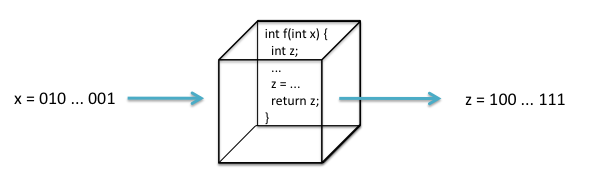
\includegraphics[width=0.8\textwidth]{computational_model_function}
\caption{The title of the Figure.}
\label{fig:fnCompModel}
\end{center}
\end{figure}



\begin{figure} [!ht] %if [h] doesn't work, we can force with !
\begin{center}
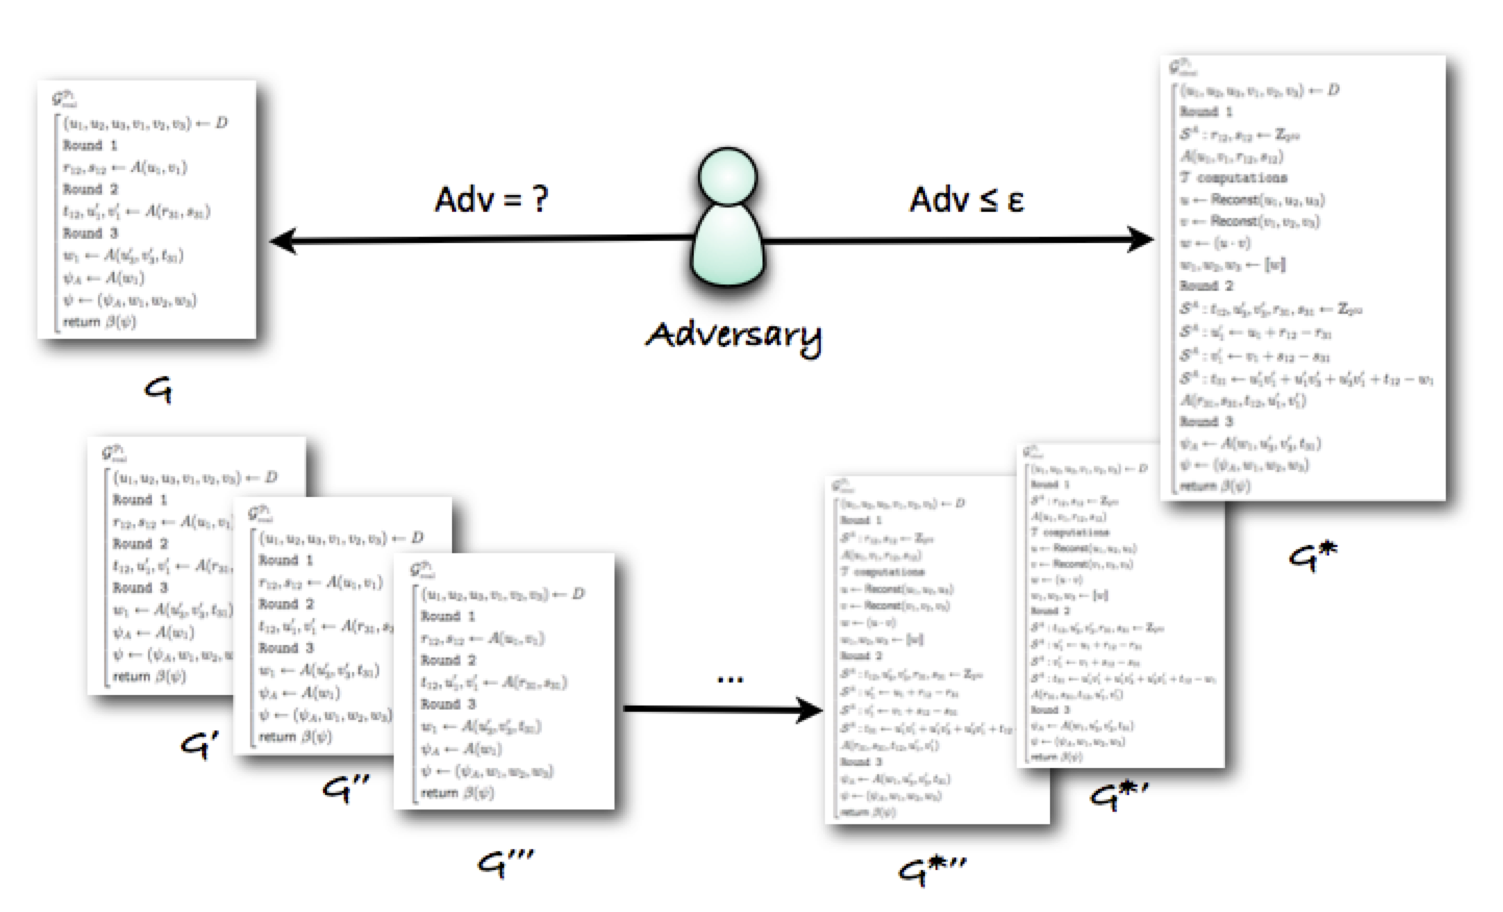
\includegraphics[width=\textwidth]{game-based_proofs}
\caption{Refer if the figure is not yours~\cite{kamm12}.}
\label{fig:game-based_proofs}
\end{center}
\end{figure}


\begin{figure} [p]
\begin{center}
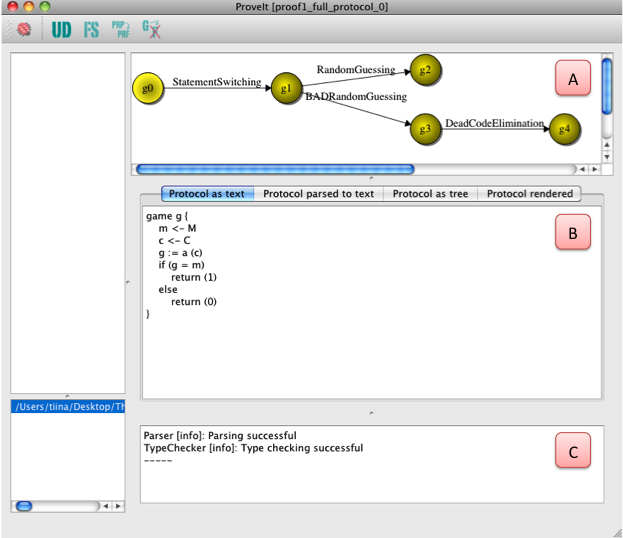
\includegraphics[width=\textwidth]{proveit_screenshot}
\caption{Screenshot of \proveit.}
\label{fig:proveit_screenshot}
\end{center}
\end{figure}

Tip: If you add a screenshot then labeling the parts might help make the text more understandable (panel C vs bottom left part), e.g.


\begin{figure} [htbp]
\begin{tabular}{c c}
%
\begin{minipage}{0.45\textwidth}
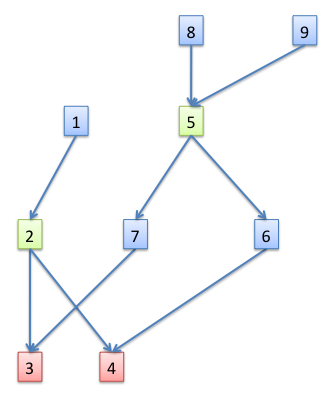
\includegraphics[width=\textwidth]{LCA_2_solutions}
\end{minipage}
%
&
\begin{minipage}{0.55\textwidth}
\centering
\begin{tabular}{ l | l |}
	Node & Decendants \\ \hline
  1 & 2, 3, 4 \\ \hline
  2 & 3, 4 \\ \hline
  3 & \\ \hline
  4 & \\ \hline
  5 & 3, 4, 6, 7 \\ \hline
  6 & 4 \\ \hline
  7 & 3 \\  \hline
  8 & 3, 4, 5, 6, 7\\ \hline
  9 & 3, 4, 5, 6, 7\\ \hline
\end{tabular}
\end{minipage}
\end{tabular}
%
\caption{Example how to put two figures parallel to each other.}
\label{fig:LCA_2_solutions}
\end{figure}


Example: A screenshot of \proveit can be seen on Figure~\ref{fig:proveit_screenshot}. The user first enters the pseudocode of the initial game in panel B. \proveit also keeps track of all the previous games showing the progress on a graph seen in panel A.

There are two figures side by side on Figure~\ref{fig:LCA_2_solutions}.



\clearpage %if newpage doesn't work
\section{Other Ways to Represent Data}

\subsection{Tables}

\begin{table}[h]
\centering
\caption{Statements in the \proveit language.}
\begin{tabular}{| l | l |}
	\hline
	\bf{Statement} & \bf{Typeset Example} \\
	\hline
	assignment & $a := 5 + b$ \\
	\hline
	uniform choice & $m <- M$ \\
	\hline
	function signature & $f : K \times M -> L$\\
	\hline
\end{tabular}
\label{tab:statements}
\end{table}


\subsection{Lists}

Numbered list example:
\begin{enumerate}
	\item item one; 
	\item item two;
	\item item three.
\end{enumerate} 

\subsection{Math mode}
Example:
\begin{equation}
a + b = c + d
\end{equation}
Aligning:
\begin{align*}
	a &= 5 \\
	b + c &= a \\
	a -2*3 &= 5/4
\end{align*}
Hint: Variables or equations in text are separated with \$ sign, e.g. $a$, $x - y$.

\paragraph{Inference Rules}
\[ 
	\inference[addition]{x : T & y : T}{x + y : T} 
\]
Bigger example:
\[
\inference[assign]{c := a + b & 
	\inference[addG]{a : \typeRat & 
		\inference[var]{b : \typeInt & \typeInt \subseteq \typeRat}{b : \typeRat}
		}{a + b : \typeRat}
	}{c : \typeRat}
\]


\subsection{algorithm2e}

\begin{algorithm} [!h]
	\caption{typeChecking} \label{alg:typeChecking}
	\KwIn{Abstract syntax tree}
	\KwResult{Type checking result; In addition, type table \typeF{type\_G} for global variables, \typeF{game} for the main game and \typeF{fun} for each $fun \in F$}
	\SetKwData{s}{s}
	\BlankLine
	
	\While{something changed in last cycle}{
		\lForEach{global statement \s} {
			\parseStatement{\s, \typeF{type\_G}}\;
		}
		\ForEach{function $fun$} {
		\lForEach{statement \s in $fun$} {
			\parseStatement{\s, \typeF{fun}}\;
		}
		}
		\lForEach{statement \s in game} {
			\parseStatement{\s, \typeF{game}}\;
		}
	}
	%\eIf{error messages were found}{\Return \False\;}{\Return \True\;}
\end{algorithm}

\subsection{Pseudocode}

\begin{figure} [htb]
\begin{lstlisting}
expression
  : NUMBER
  | VARIABLE
  | '+' expression
  | expression '+' expression
  | expression '*' expression
  | function_name '(' parameters ')'
  | '(' expression ')'
\end{lstlisting}
\caption{Grammar of arithmetic expressions.}
\label{fig:parser_exp}
\end{figure}

\subsection{Frame Around Information}

Tip: We can use minipage to create a frame around some important information.
\begin{figure} [h]
\frame{
\begin{minipage}{\textwidth}
\begin{enumerate}
	\item integer division ($\opDiv$) -- only usable between \typeInt types
	\item remainder ($\%$) -- only usable between \typeInt types
\end{enumerate}
\end{minipage}
}
\caption{Arithmetic operations in \proveit revisited.}
\label{fig:aritmOp_revisit}
\end{figure}



\clearpage
\section{Conclusion}

\TODO{what did you do?} 
\TODO{What are the results?}
\TODO{future work?}

\newpage

% BibTeX bibliography
\bibliographystyle{alpha} %plain=[1], alpha=[BGZ09]
\bibliography{bachelor-thesis}

\addcontentsline{toc}{section}{\refname}


% Use Biblatex if you have problems with Estonian keywords
%\printbibliography %biblatex


\newpage
%\appendix
%\section*{\appendixname}
\iflanguage{english}%
  {\section*{Appendix}
  \addcontentsline{toc}{section}{Appendix}
  }%
  {\section*{Lisad}
  \addcontentsline{toc}{section}{Lisad}}


\section*{I. Glossary}
\addcontentsline{toc}{subsection}{I. Glossary}

\newpage

%=== Licence in English
\newcommand{\licencehint}[2]{\\\hspace*{#1}\textsl(#2)\par}
\newcommand\EngLicence{{%
\selectlanguage{english}
\section*{II. Licence}

\addcontentsline{toc}{subsection}{II. Licence}

\subsection*{Non-exclusive licence to reproduce thesis and make thesis public}

I, \textbf{Alice Cooper}, %author's name
  \licencehint{10mm}{author's name}

\begin{enumerate}
\item
herewith grant the University of Tartu a free permit (non-exclusive licence) to
\par
reproduce, for the purpose of preservation, including for adding to the DSpace digital archives until the expiry of the term of copyright,
\par
\textbf{Type Inference for Fourth Order Logic Formulae}, %
  \licencehint{10mm}{title of thesis}
\par
supervised by Axel Rose and May Flower. %supervisor's name
  \licencehint{10mm}{supervisor's name}
\item
I grant the University of Tartu a permit to make the work specified in p. 1 available to the public via the web environment of the University of Tartu, including via the DSpace digital archives, under the Creative Commons licence CC BY NC ND 3.0, which allows, by giving appropriate credit to the author, to reproduce, distribute the work and communicate it to the public, and prohibits the creation of derivative works and any commercial use of the work until the expiry of the term of copyright.
\item
I am aware of the fact that the author retains the rights specified in p. 1 and 2.
\item
I certify that granting the non-exclusive licence does not infringe other persons' intellectual property rights or rights arising from the personal data protection legislation. 
\end{enumerate}

\noindent
Alice Cooper\\ %author's name
\textbf{\textsl{dd/mm/yyyy}}
}}%\newcommand\EngLicence


%=== Licence in Estonian
\newcommand\EstLicence{{%
\selectlanguage{estonian}
\section*{II. Litsents}

\addcontentsline{toc}{subsection}{II. Litsents}

\subsection*{Lihtlitsents lõputöö reprodutseerimiseks ja üldsusele kättesaadavaks tegemiseks}

Mina, \textbf{Alice Cooper}, %author's name
  \licencehint{10mm}{autori nimi}

\begin{enumerate}
\item
annan Tartu Ülikoolile tasuta loa (lihtlitsentsi) minu loodud teose
\par
\textbf{Tüübituletus neljandat järku loogikavalemitele}, %title of thesis
    \licencehint{10mm}{lõputöö pealkiri}
\par
mille juhendaja(d) on Axel Rose ja May Flower, %supervisor's name(s)
  \licencehint{10mm}{juhendaja nimi}
\par
reprodutseerimiseks eesmärgiga seda säilitada, sealhulgas lisada digitaalarhiivi DSpace kuni autoriõiguse kehtivuse lõppemiseni.
\par
\item
Annan Tartu Ülikoolile loa teha punktis 1 nimetatud teos üldsusele kättesaadavaks Tartu Ülikooli veebikeskkonna, sealhulgas digitaalarhiivi DSpace kaudu Creative Commonsi litsentsiga CC BY NC ND 3.0, mis lubab autorile viidates teost reprodutseerida, levitada ja üldsusele suunata ning keelab luua tuletatud teost ja kasutada teost ärieesmärgil, kuni autoriõiguse kehtivuse lõppemiseni.
\item
Olen teadlik, et punktides 1 ja 2 nimetatud õigused jäävad alles ka autorile.
\item
Kinnitan, et lihtlitsentsi andmisega ei riku ma teiste isikute intellektuaalomandi ega isikuandmete kaitse õigusaktidest tulenevaid õigusi. 
\end{enumerate}

\noindent
Alice Cooper\\ %author's name
\textbf{\textsl{pp.kk.aaaa}}
}}%\newcommand\EstLicence


%===Choose the licence in active language
\iflanguage{english}{\EngLicence}{\EstLicence}


\end{document}

